%! Author = sbbfti
%! Date = 10/06/2020


\section{Results}\label{sec:results}

\subsection{Comfort DB overview}\label{subsec:comfort-db-overview}

A total of \var{entries_db_used} entries met the inclusion criteria listed in the Methodology Section.
The distribution of the six input variables used to calculate the PMV indices is depicted in Figure~\ref{fig:dist_input_data}.

\begin{figure}
    \centering
    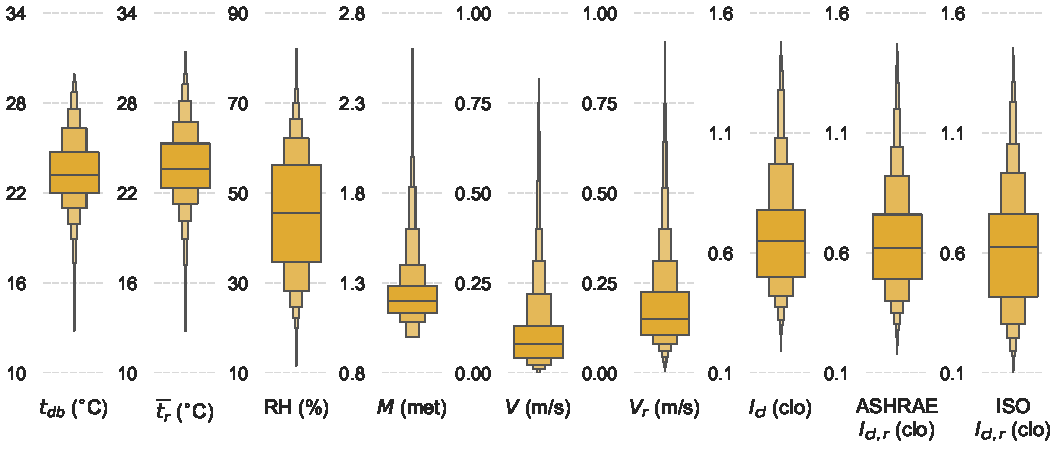
\includegraphics[width=\textwidth]{figures/dist_input_data}
    \caption{Distribution of the input variables used to calculate the \ac{pmv} values.
    The data are shown using boxen-plots (letter-value plots).
    They depict the median as the centerline and each successive level outward contains half of the remaining data.}
    \label{fig:dist_input_data}
\end{figure}

Figure~\ref{fig:dist_other_data} shows the distribution of the age, height, weight, and running mean outdoor temperature grouped by sex.
Less than half (\num{23300}) of the total entries had information about the participant's sex.
Out of those data were almost equally distributed among male \qty{52}{\percent} and females.
Ages are not normally distributed, the same is true for the running mean outdoor temperature.
About half of the participants (\qty{52}{\percent}) were aged between \num{20} and \num{35} years old.
While \qty{56}{\percent} of the running mean outdoor temperature values where between \qtyrange{10}{25}{\celsius}.
Mens were significantly heavier and taller than females.

\begin{figure}
    \centering
    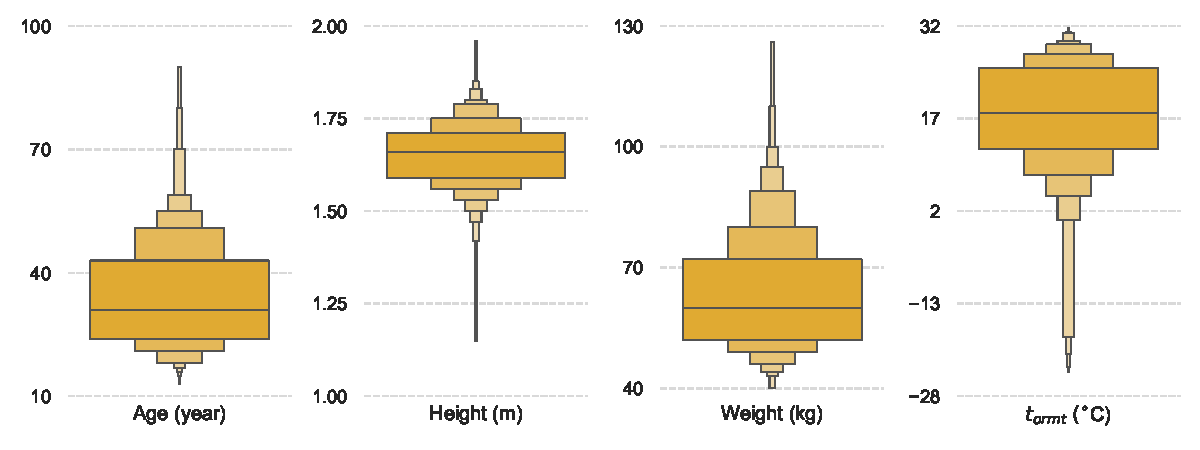
\includegraphics[width=\textwidth]{figures/dist_other_data}
    \caption{Distribution of age, height, weight, and running mean outdoor temperature.
    The data are grouped by sex.}
    \label{fig:dist_other_data}
\end{figure}

Figure~\ref{fig:bar_plot_tp_by_ts} shows on the left the percentage of thermal preference votes grouped by each \ac{tsv}.
The left Figure also reports the number of points for each \ac{tsv}.
Only \var{entries_with_tp} that had information about the thermal preference.
Thus, on the right we show a bar chart depicting the distribution of all the \ac{tsv} votes, we have used in the analysis.
The \gls{db2} in respect to the \ac{tsv} is unbalanced.
Approximately \var{perc_tsv_neutral} of all the entries have a \ac{tsv} of `Neutral'.
While less than \var{perc_tsv_hot} of the total sample of participants reported to be either `Hot' or `Cold'.
In the \gls{db2} more than \qty{50}{\percent} of participants who were either `slightly warm' or `slightly cool' wanted to be `cooler' or `warmer', respectively.
However, in thermal comfort research it is generally assumed that people who are `slightly warm' or `slightly cool' are thermally comfortable.
This finding challenges the above assumption.
Moreover, these results provide additional evidence that the use of the thermal preference scale is better suited to determine how people perceive their thermal environment.
The thermal sensation vote clearly allows to determine whether participants would take action or not to modify their current thermal environment.
The \ac{tsv}, on the contrary, does not allow to determine which actions should be taken to increase thermal comfort conditions for occupants.

\begin{figure}
    \centering
    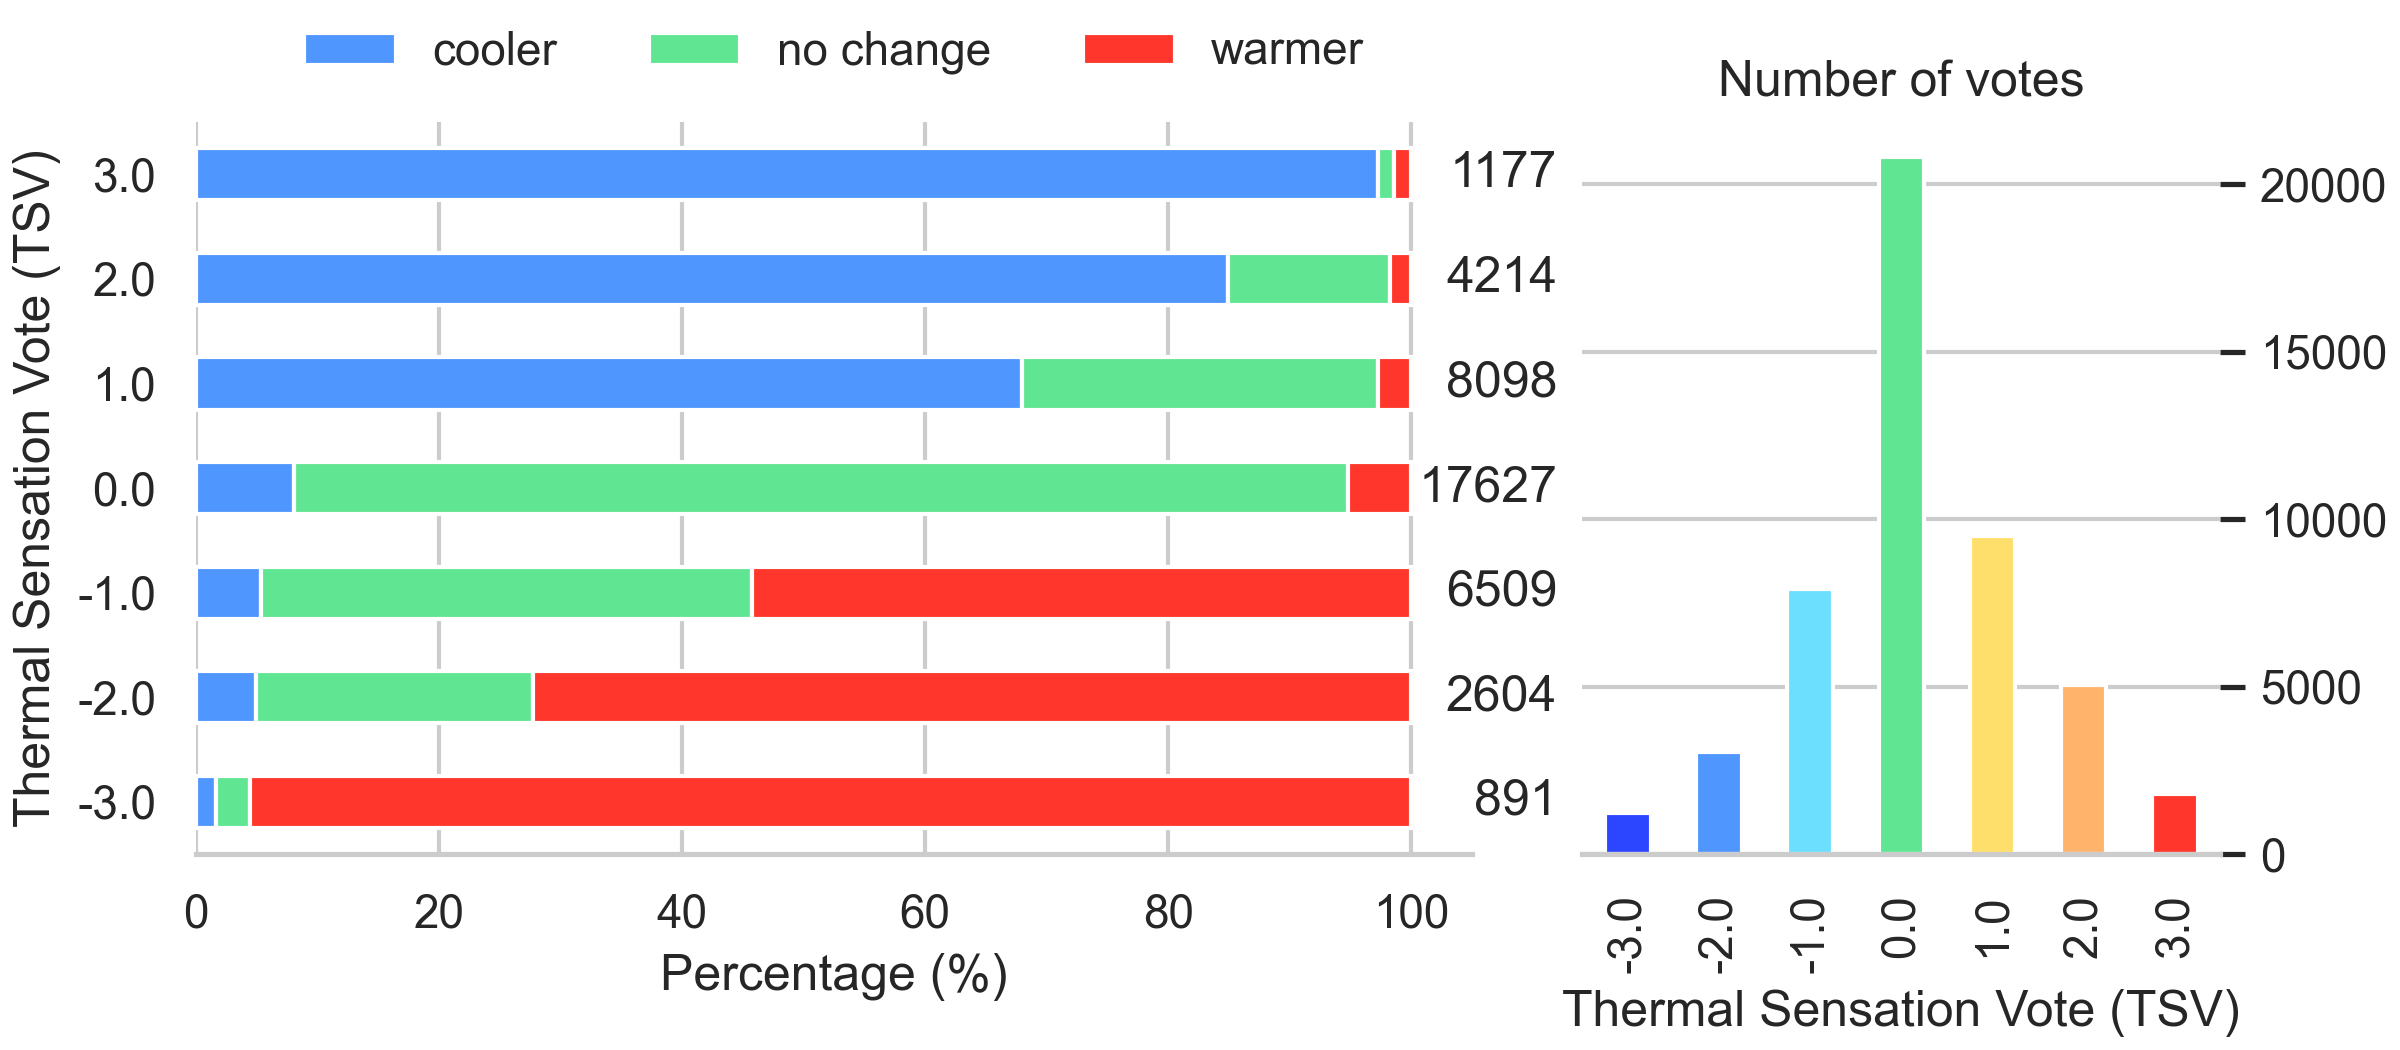
\includegraphics[width=\textwidth]{figures/bar_plot_tp_by_ts}
    \caption{The left Figure shows the percentage of thermal preference votes for each thermal sensation vote.
    The numbers on the right side of each bar show the number of points for each \ac{tsv}.
    The right figure shows the total number of data points grouped by \ac{tsv}.
    Each bin in the Figure of the right has more data points than in the Figure on the left since information about the occupants thermal preference were not always available.}
    \label{fig:bar_plot_tp_by_ts}
\end{figure}

\begin{figure}
    \centering
    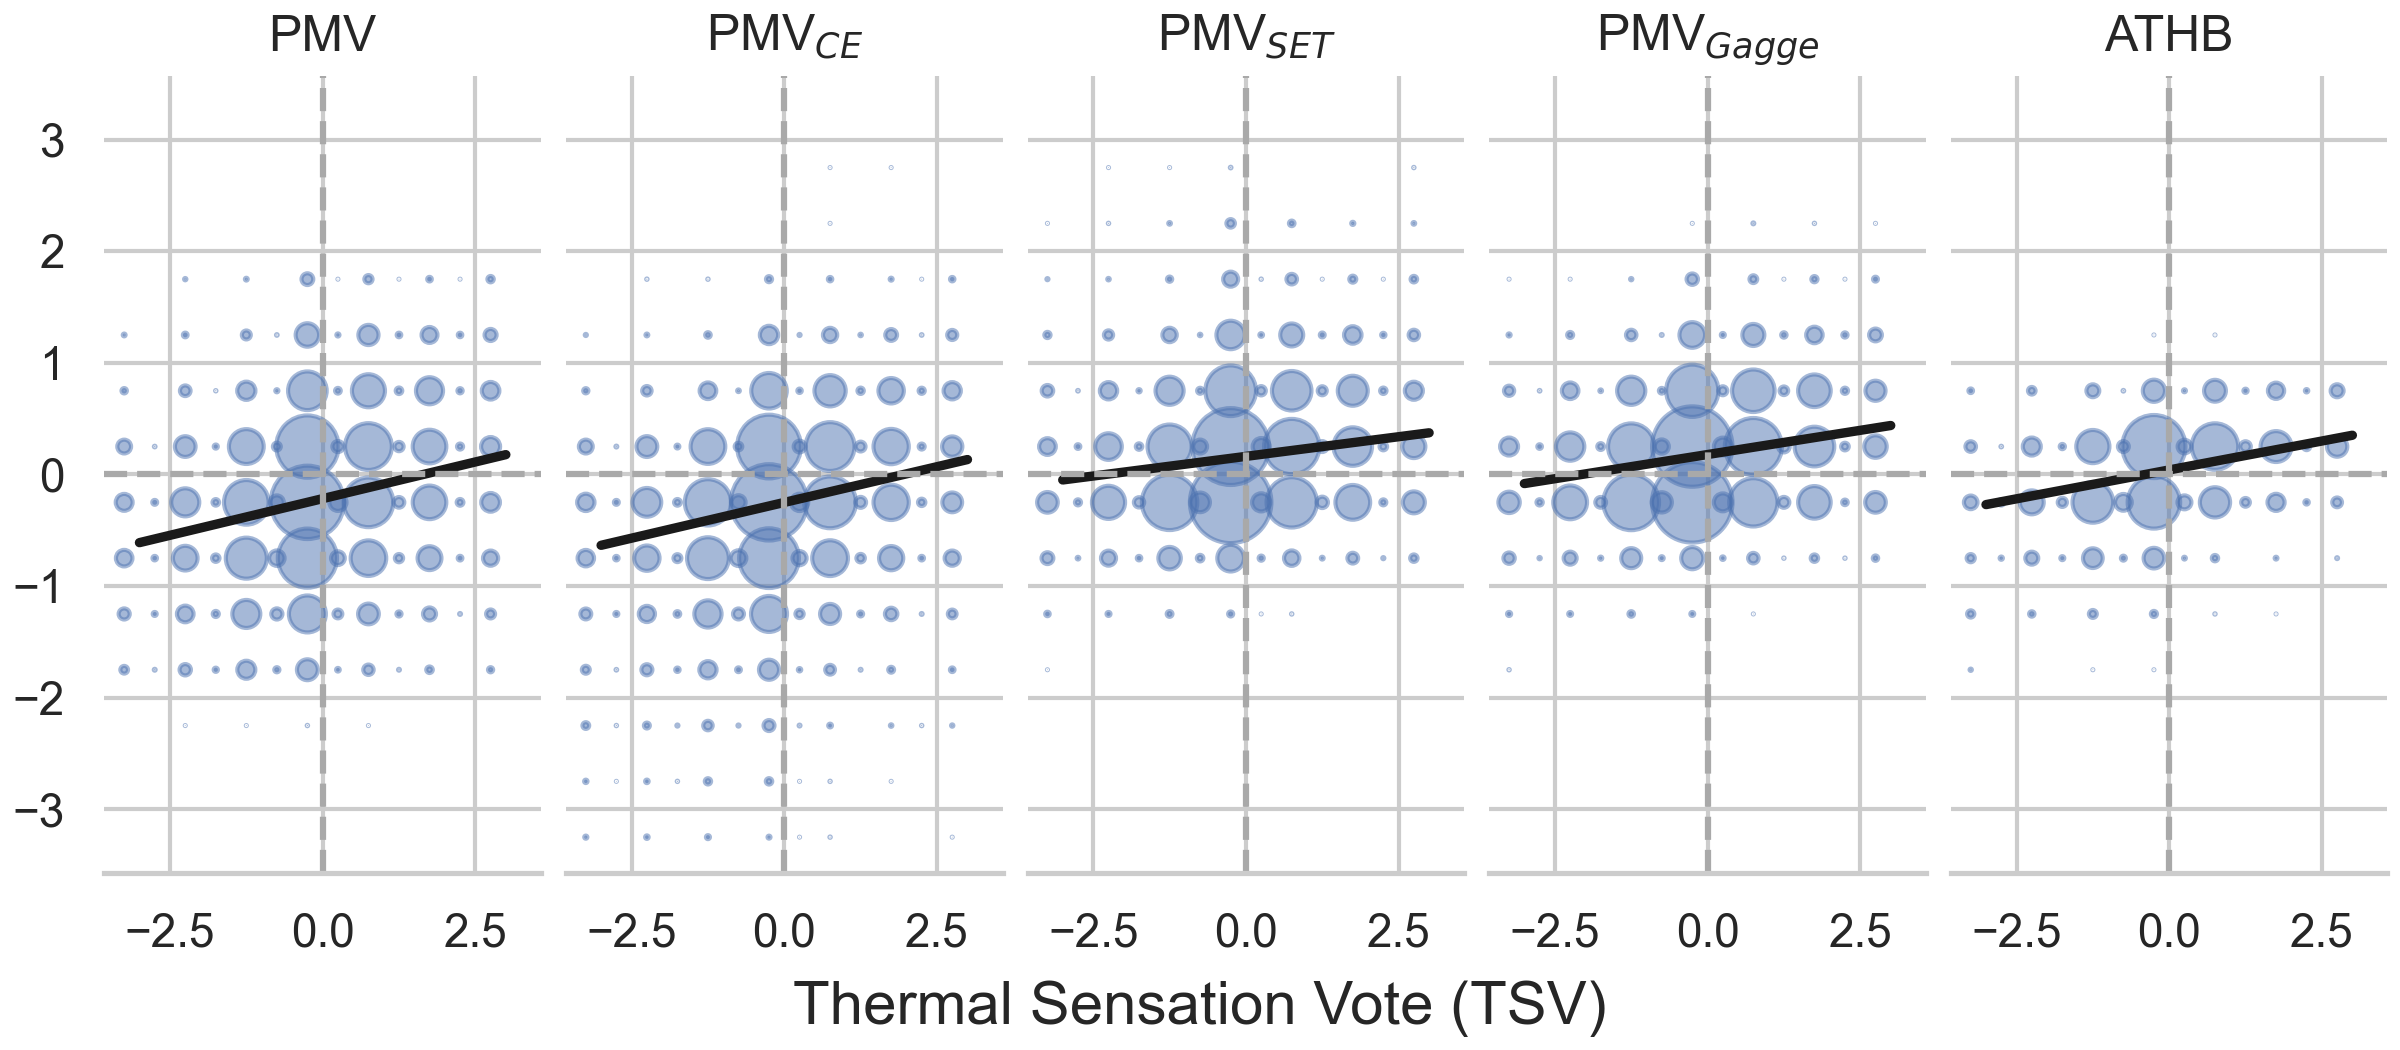
\includegraphics[width=\textwidth]{figures/bubble_models_vs_tsv}
    \caption{}
    \label{fig:bubble_models_vs_tsv}
\end{figure}

\begin{figure}
    \centering
    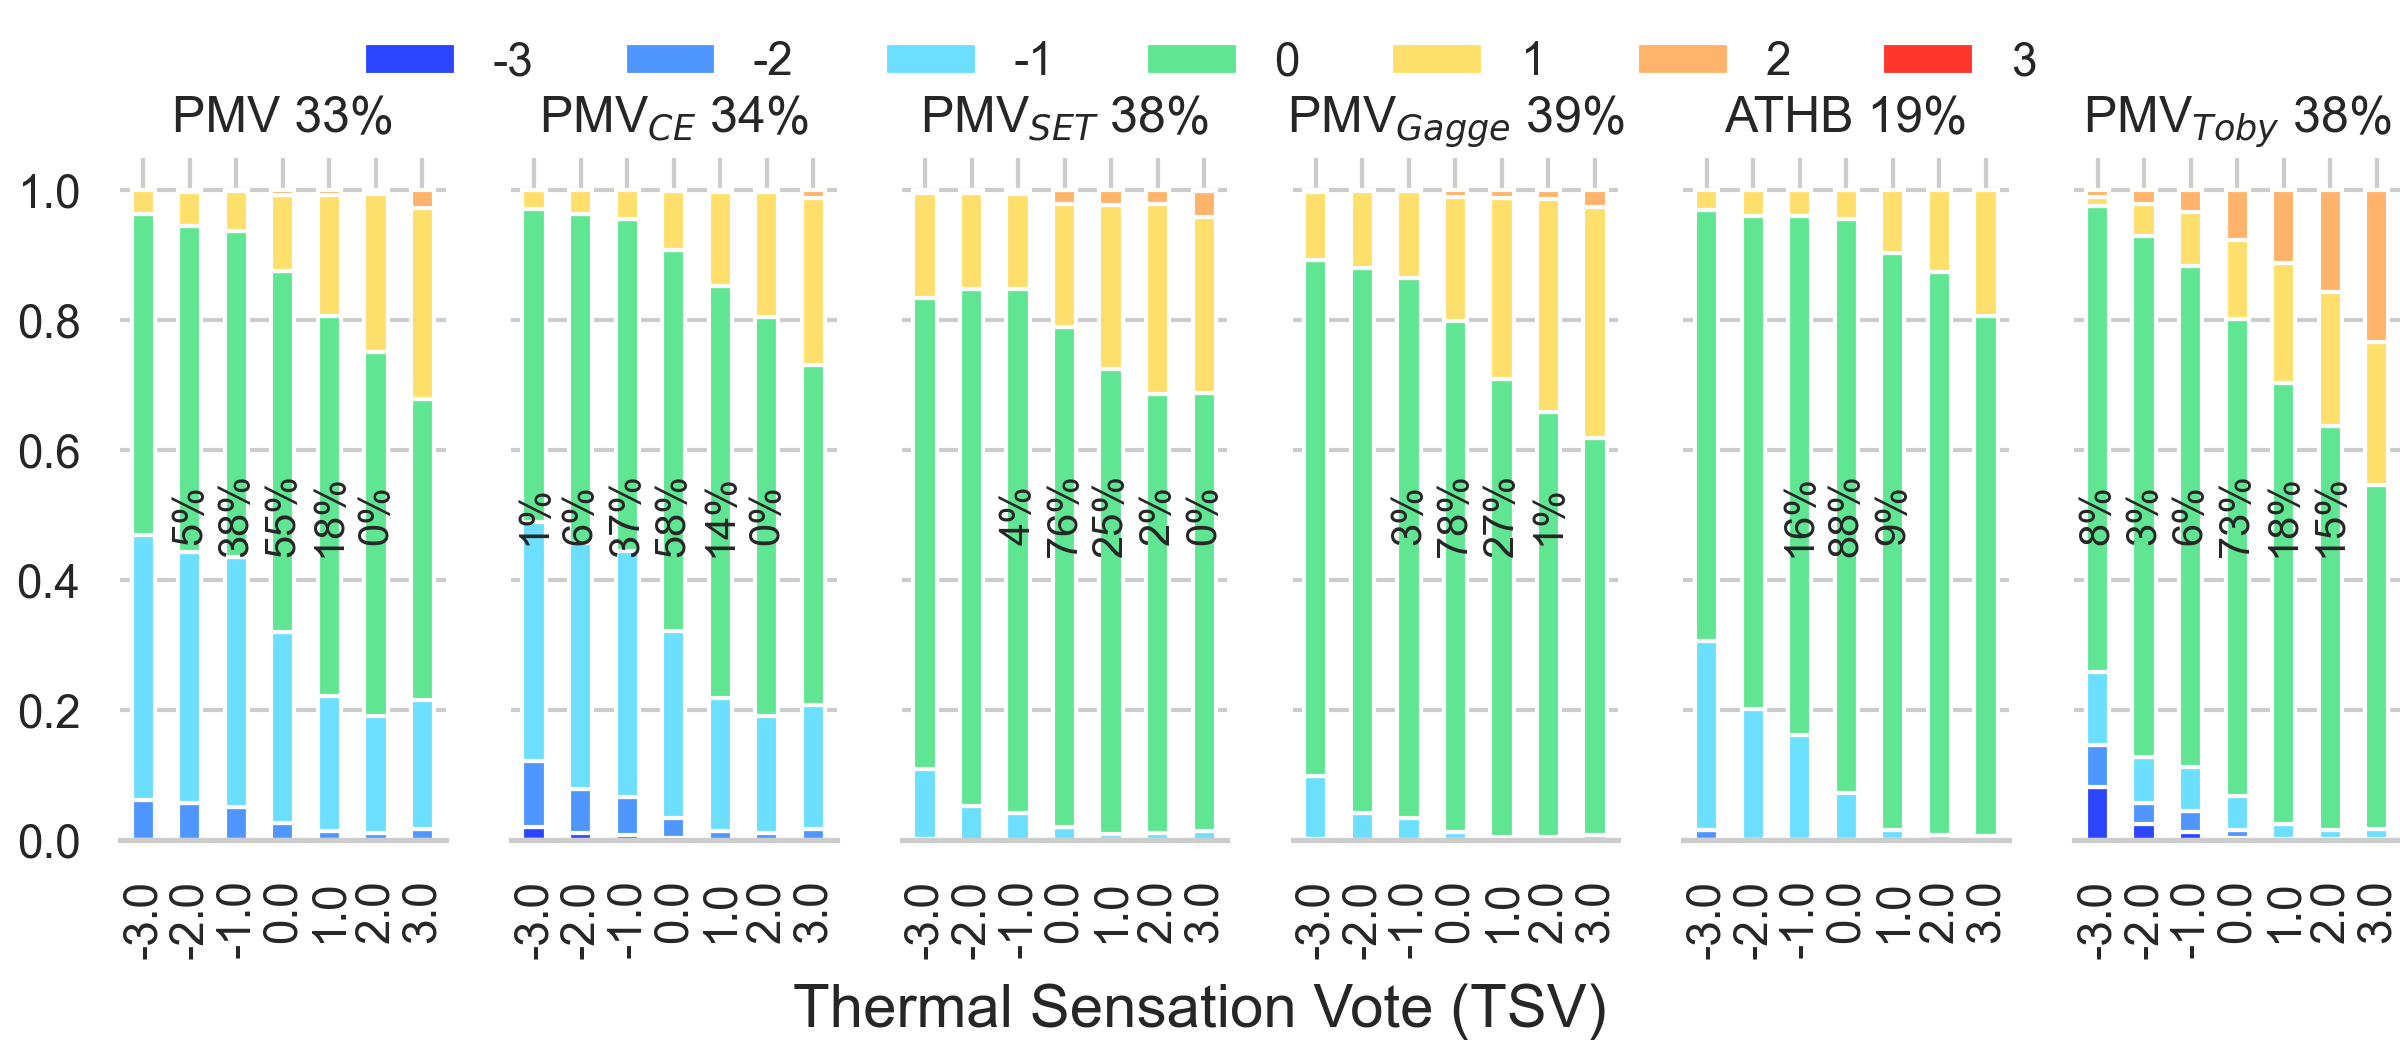
\includegraphics[width=\textwidth]{figures/bar_stacked_model_accuracy}
    \caption{}
    \label{fig:bar_stacked_model_accuracy}
\end{figure}

\begin{figure}
    \centering
    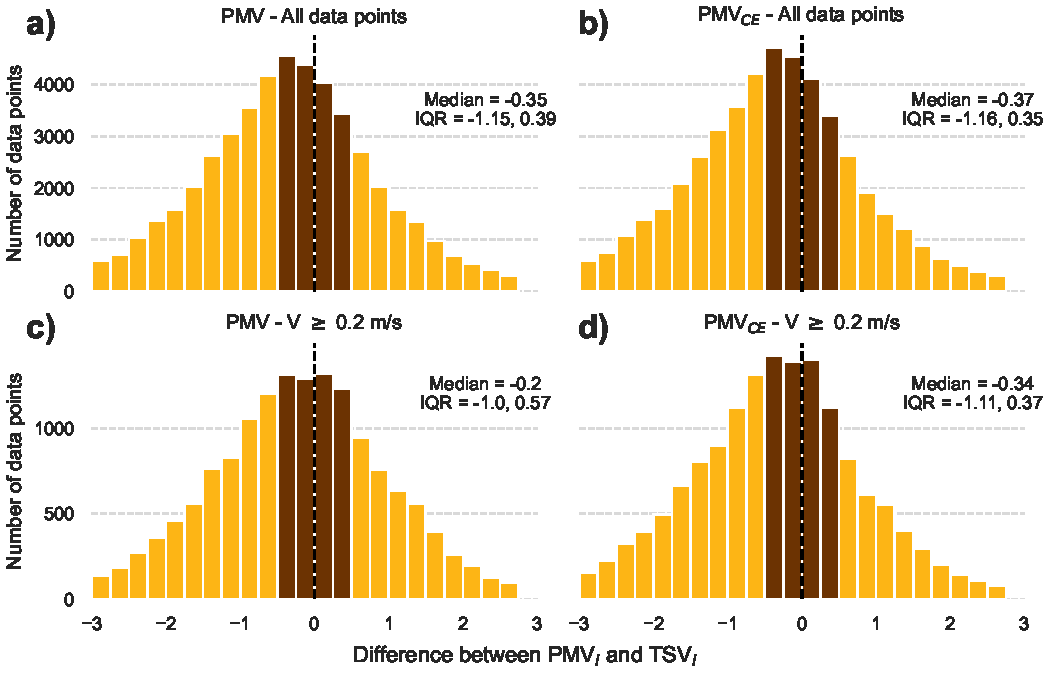
\includegraphics[width=\textwidth]{figures/hist_discrepancies}
    \caption{}
    \label{fig:hist_discrepancies}
\end{figure}

\begin{figure}
    \centering
    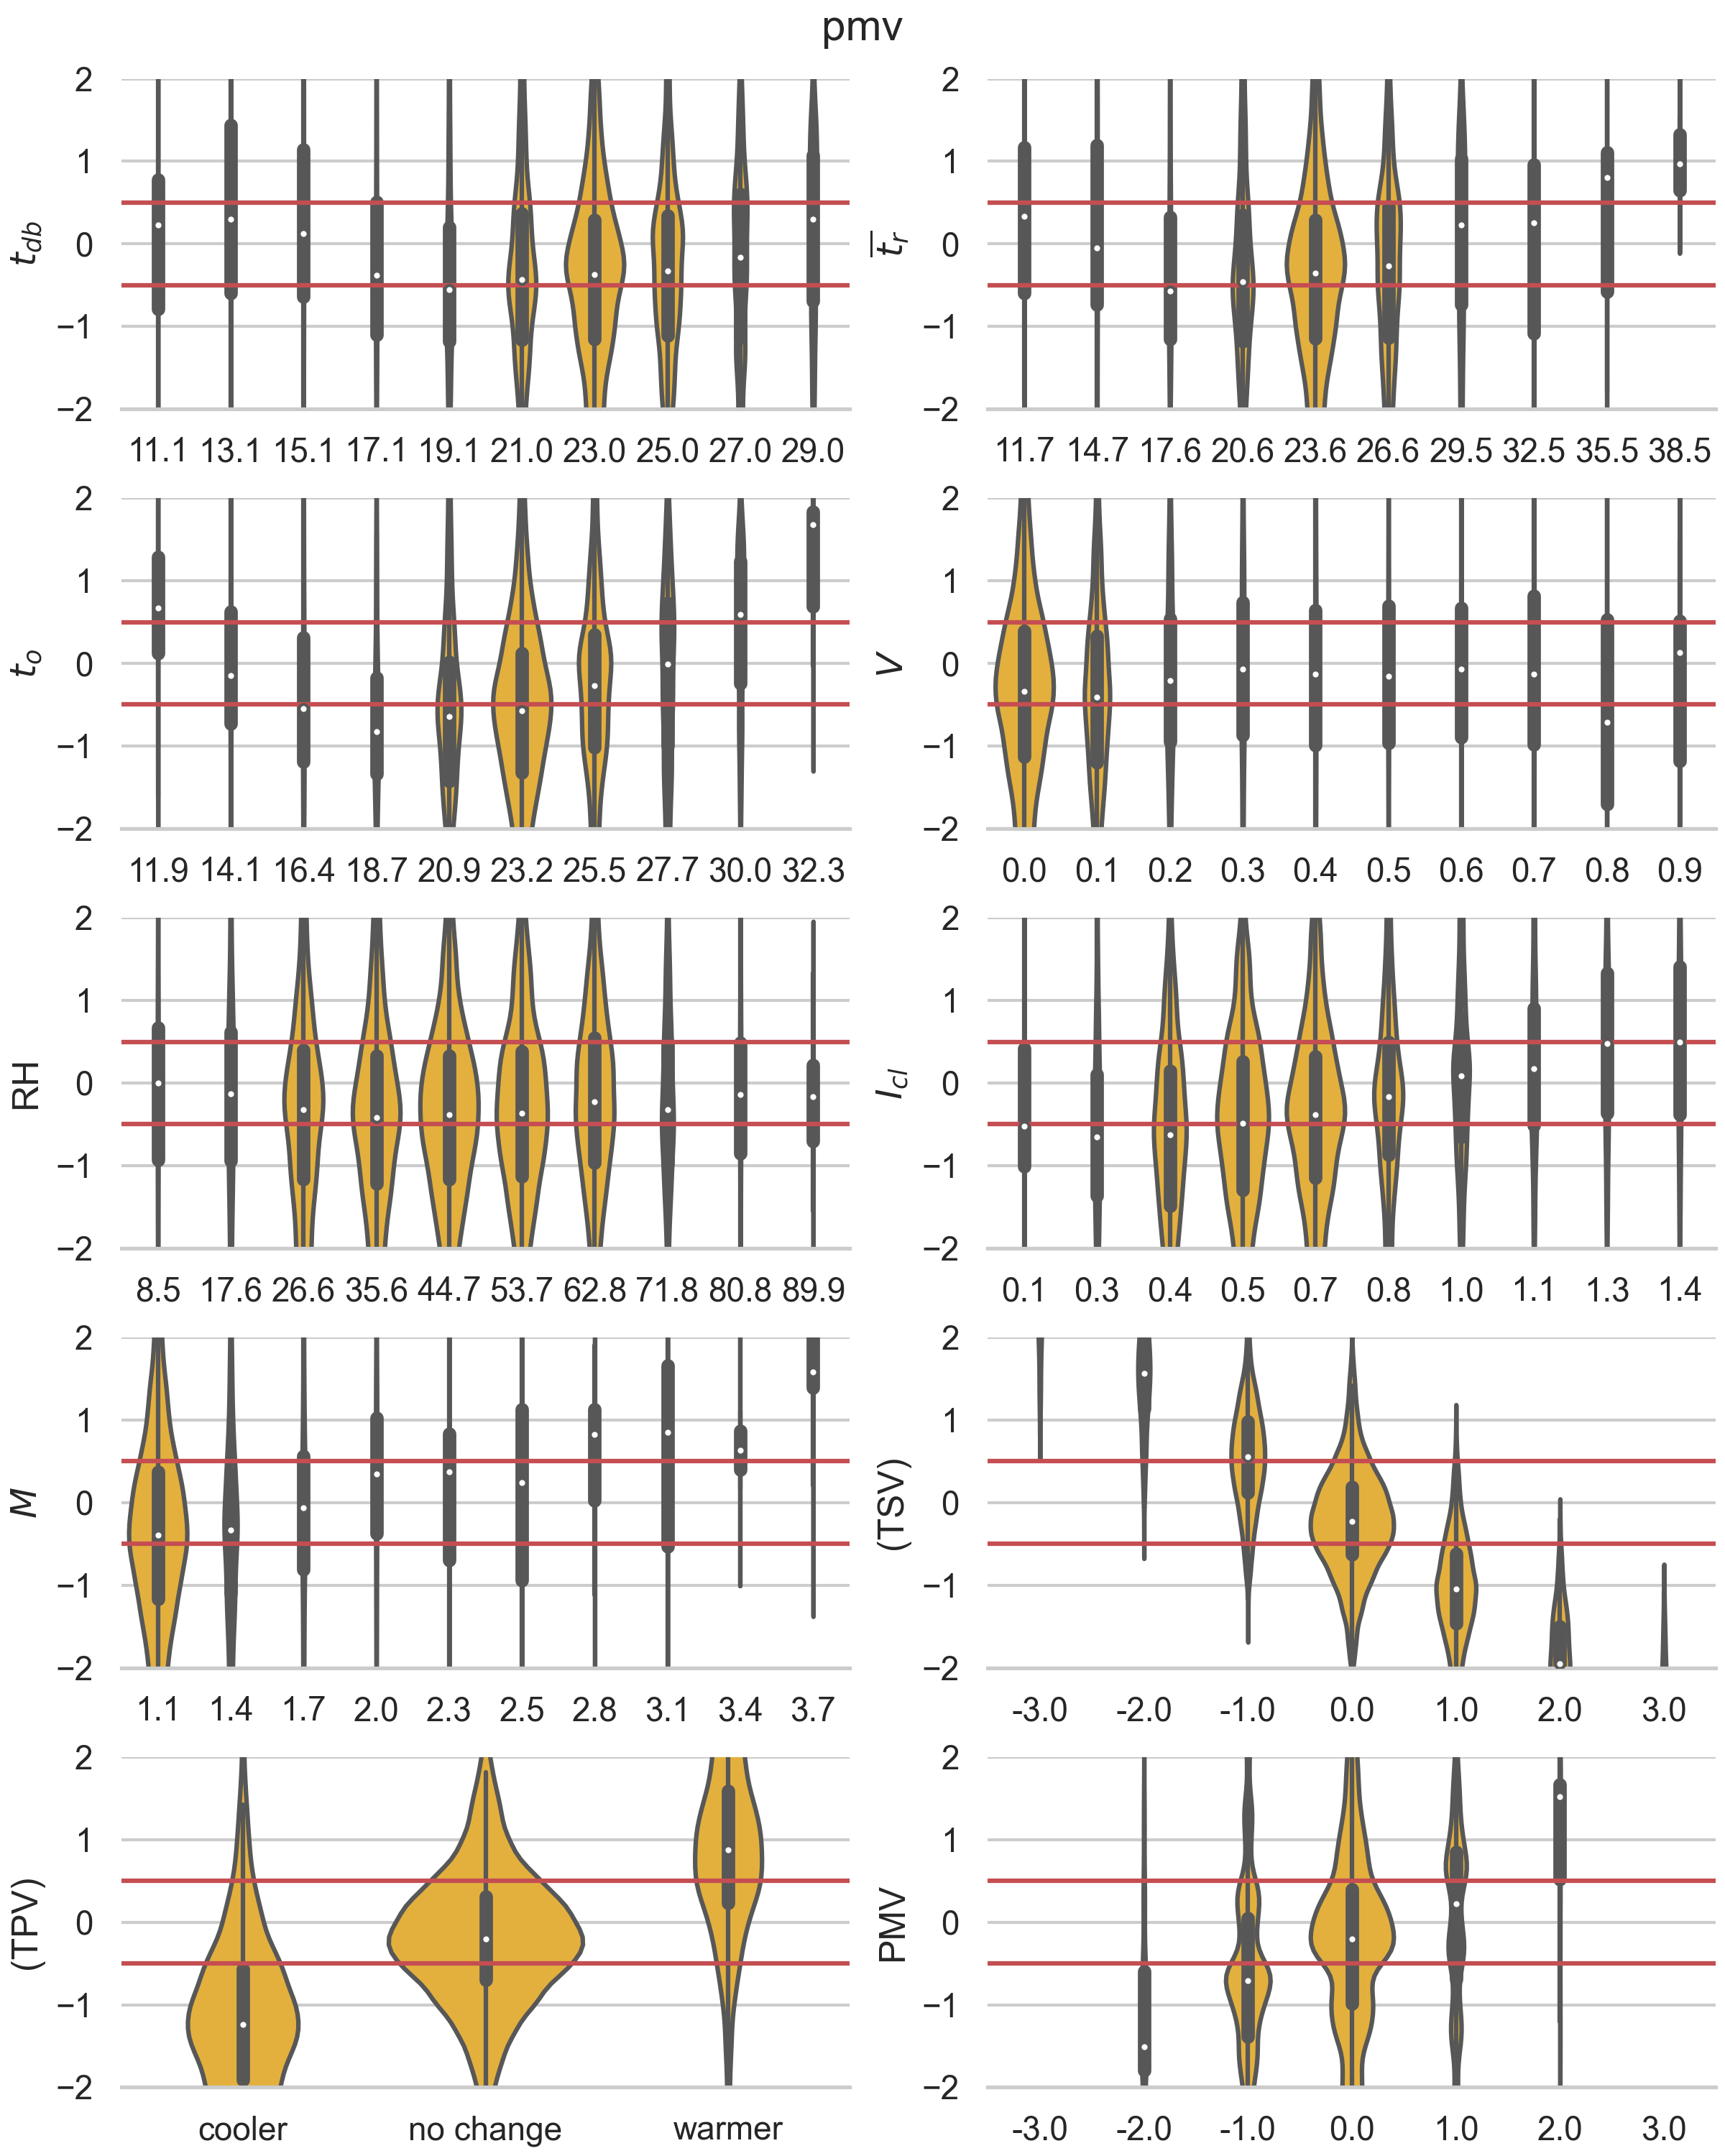
\includegraphics[width=\textwidth]{figures/bias_pmv}
    \caption{}
    \label{fig:bias_pmv}
\end{figure}

\begin{figure}
    \centering
    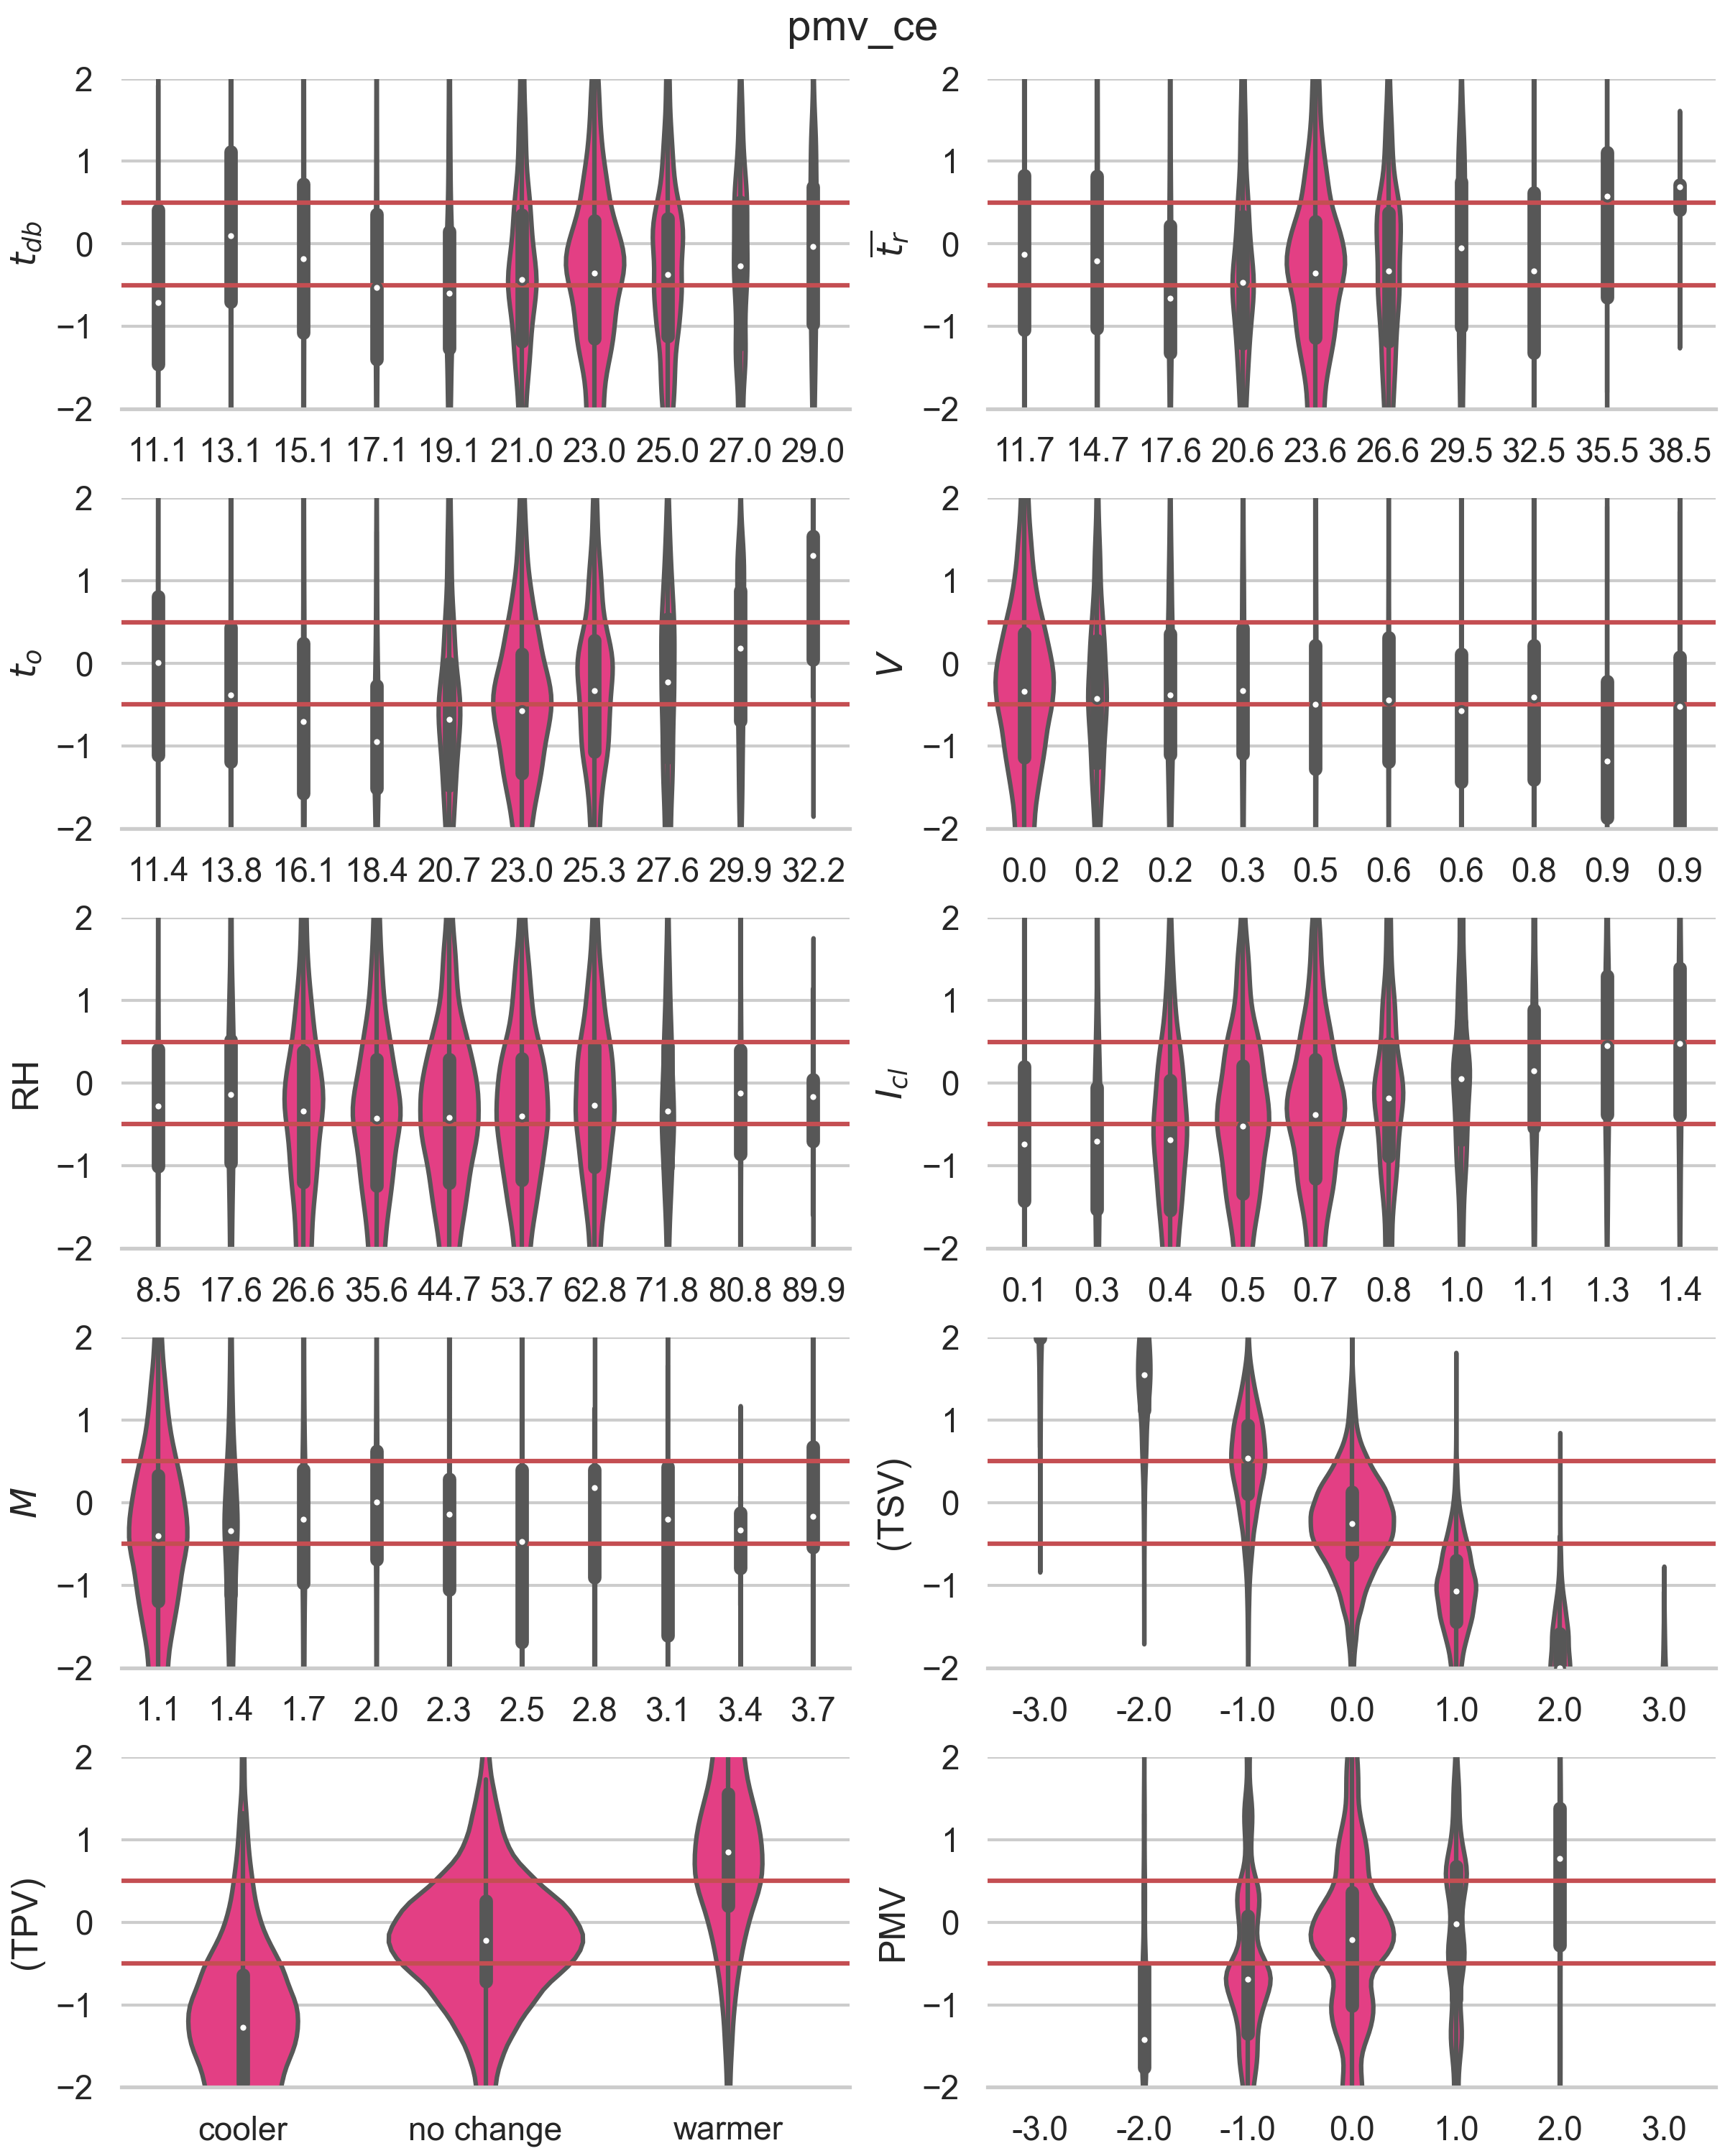
\includegraphics[width=\textwidth]{figures/bias_pmv_ce}
    \caption{}
    \label{fig:bias_pmv_ce}
\end{figure}

\begin{figure}
    \centering
    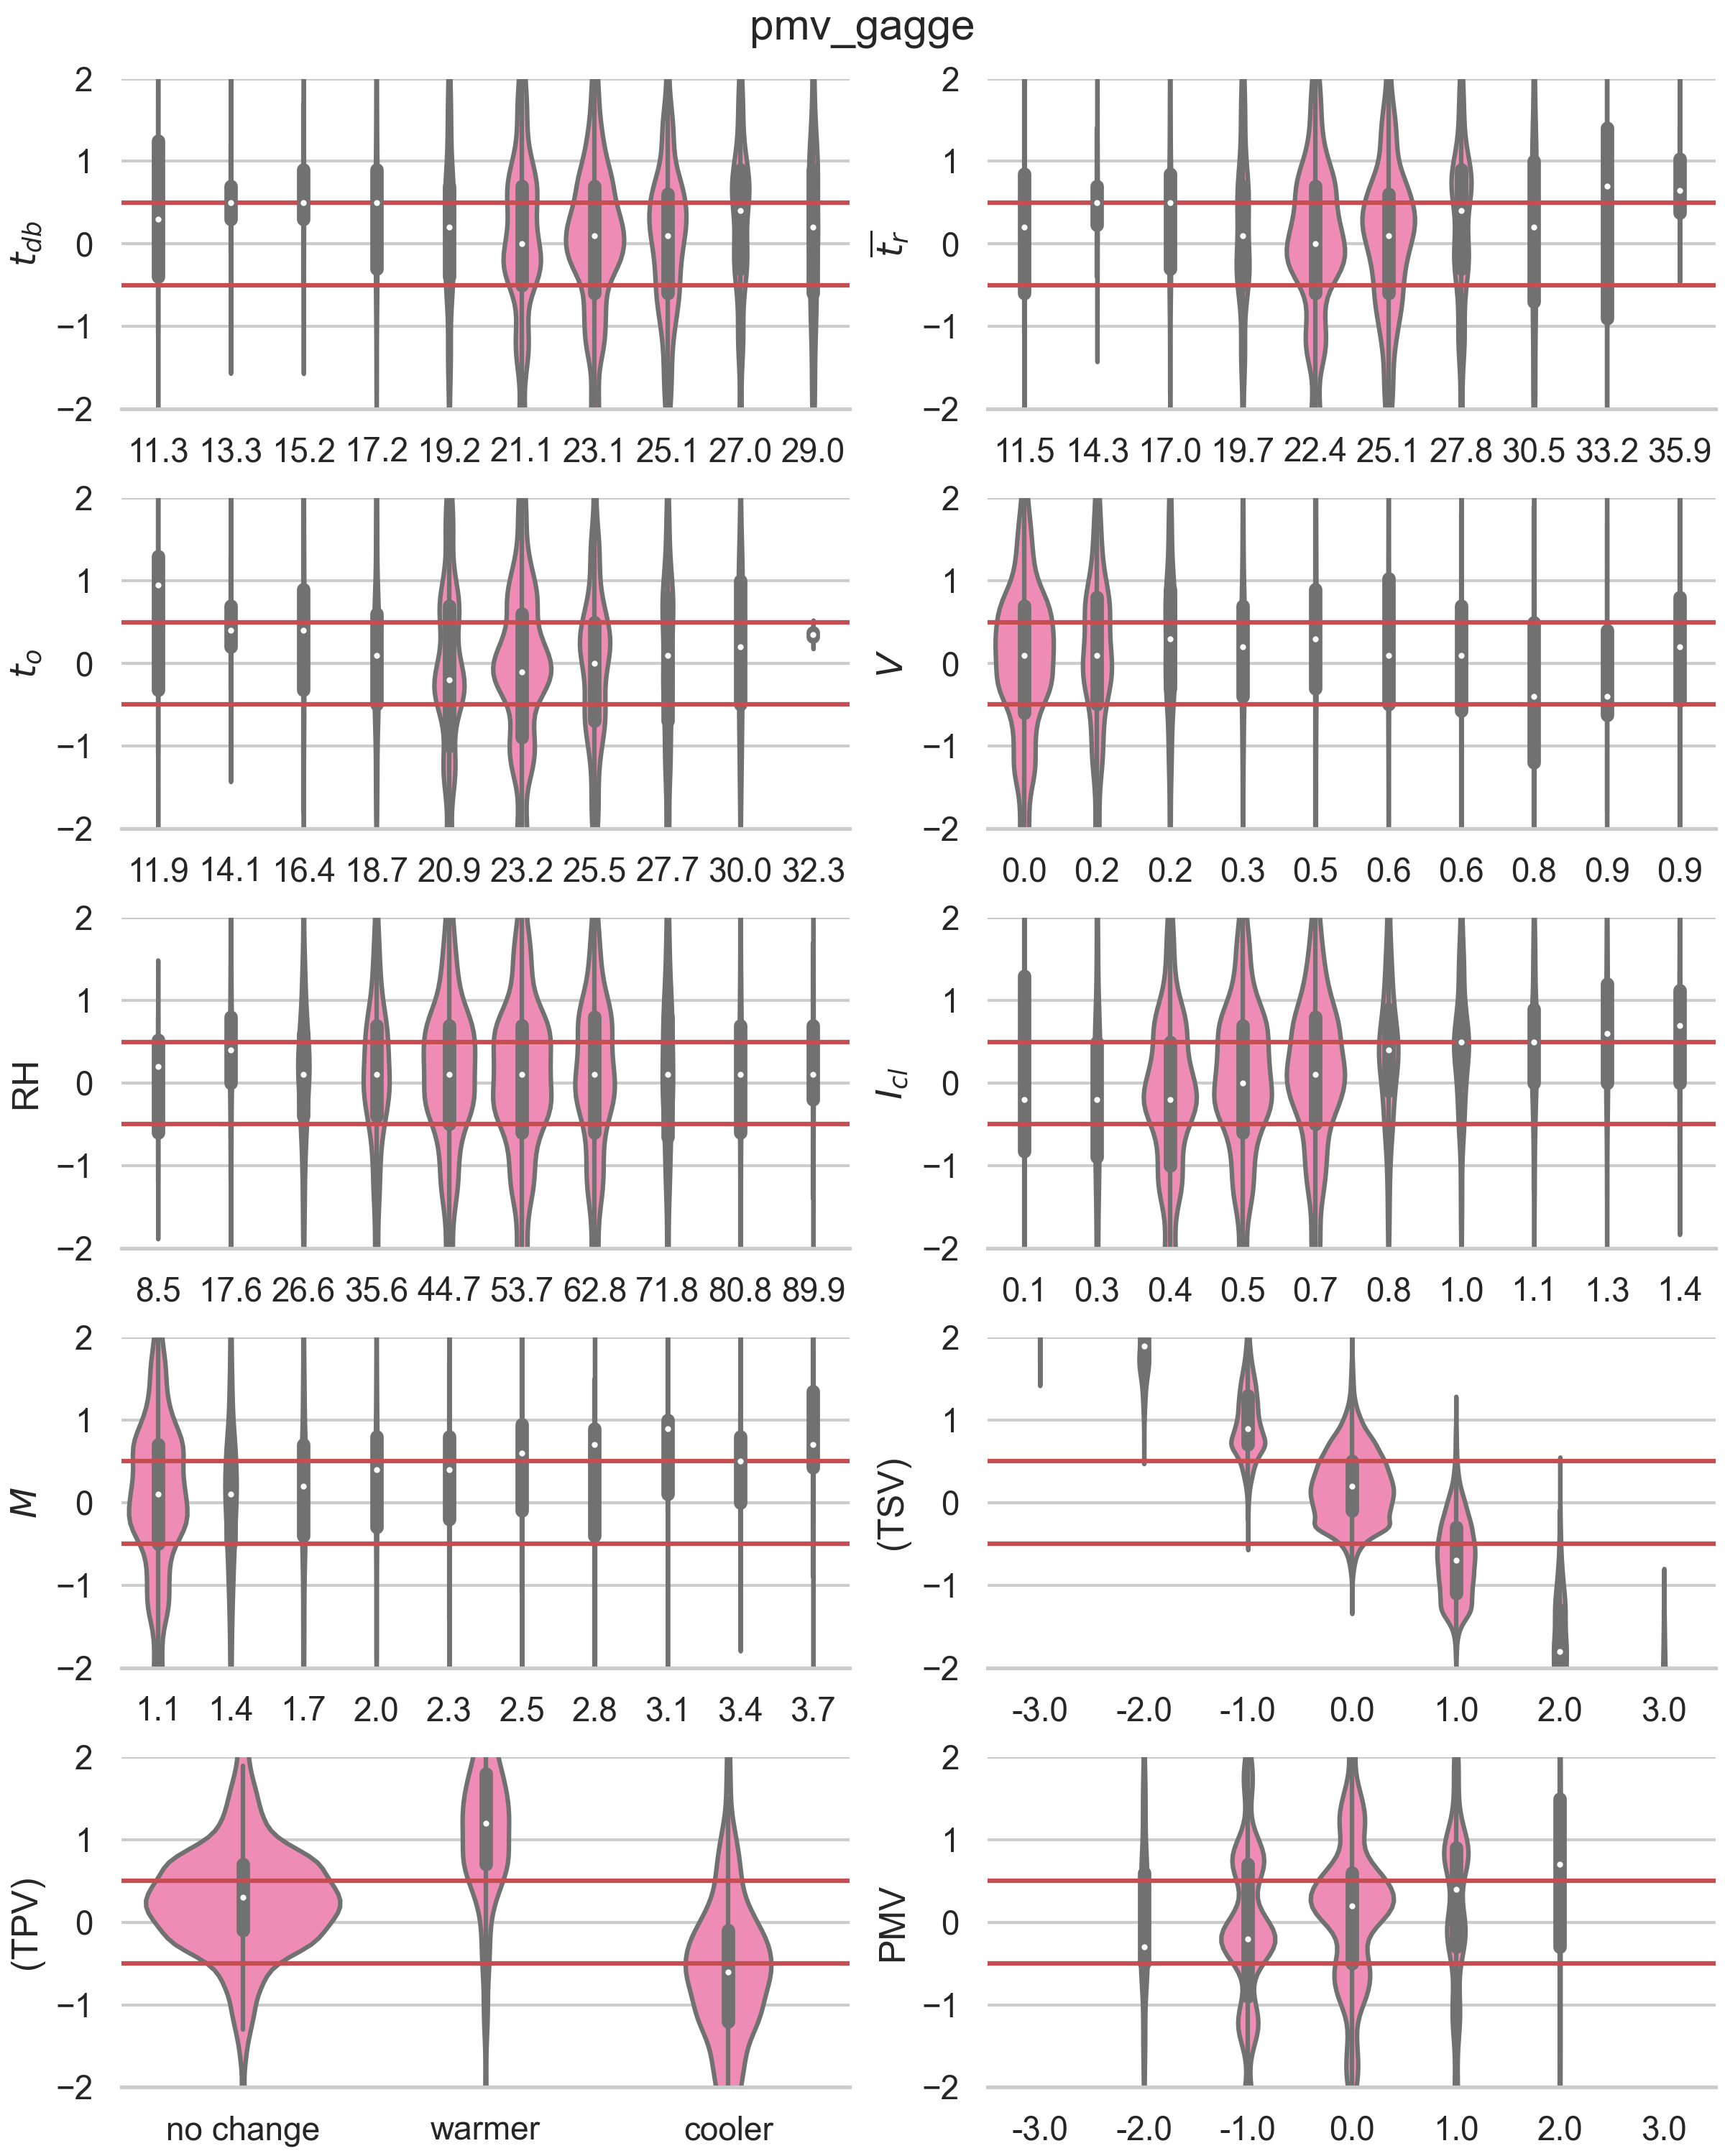
\includegraphics[width=\textwidth]{figures/bias_pmv_gagge}
    \caption{}
    \label{fig:bias_pmv_gagge}
\end{figure}

\begin{figure}
    \centering
    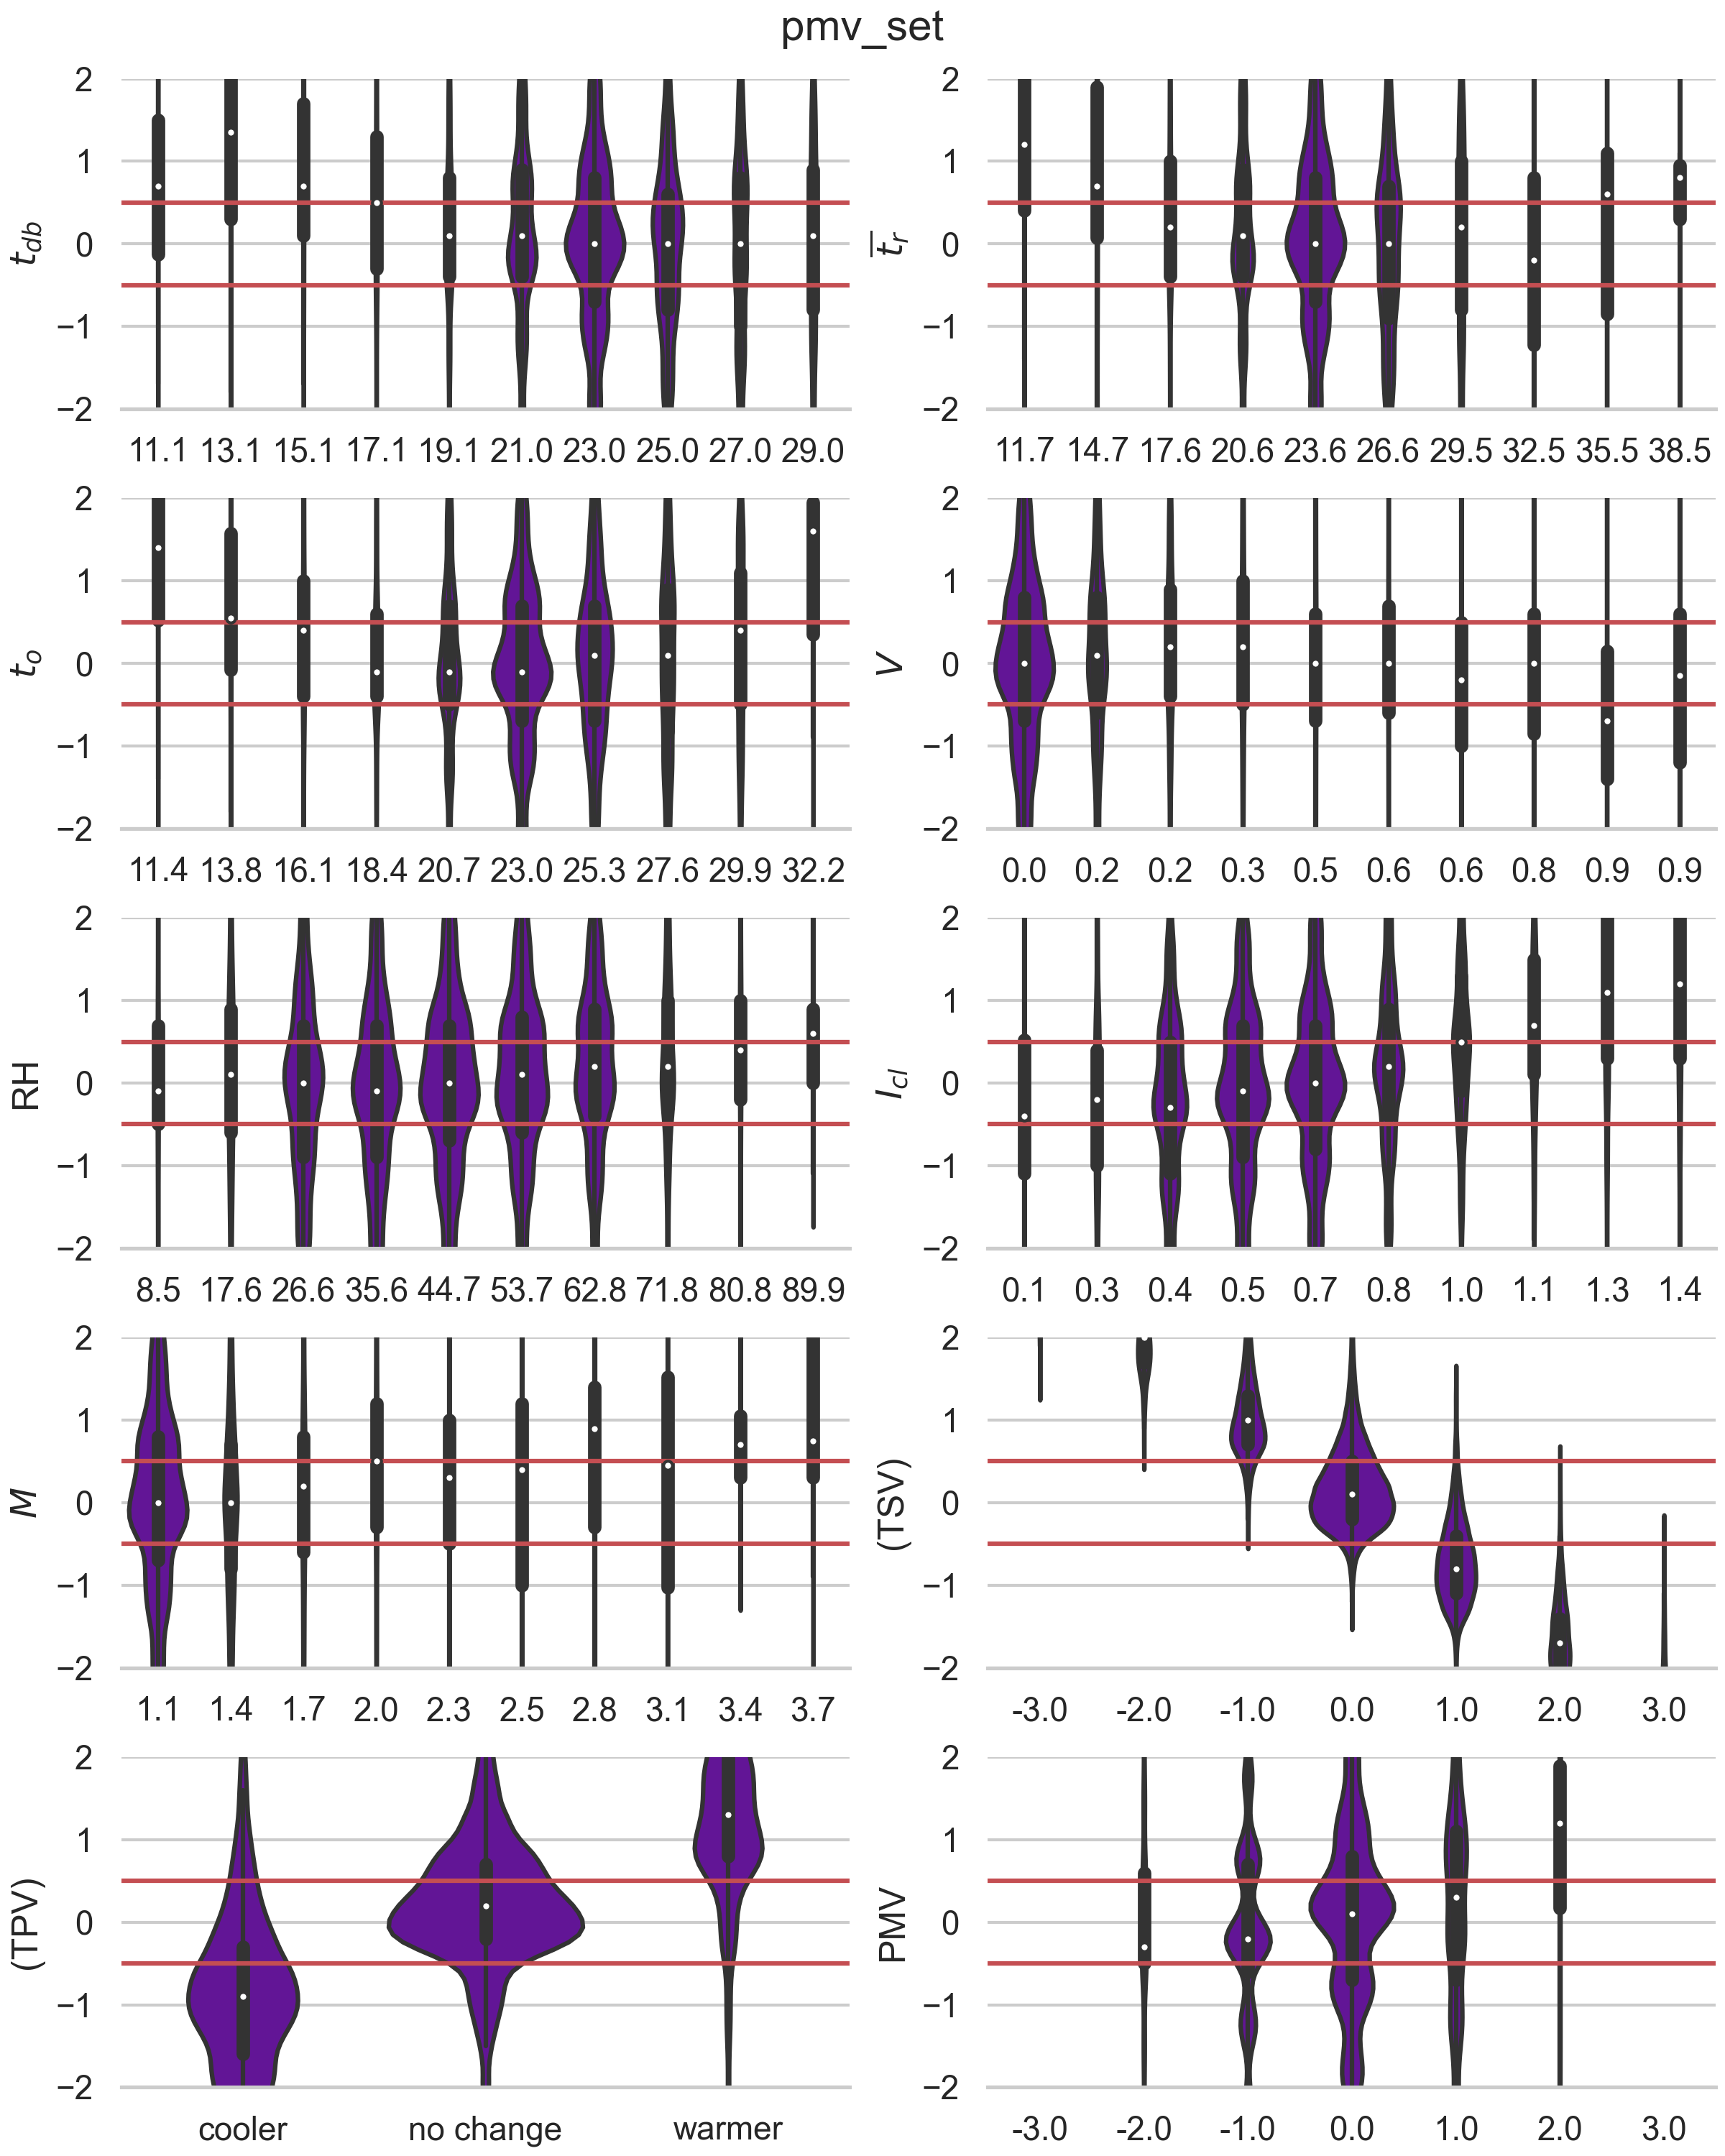
\includegraphics[width=\textwidth]{figures/bias_pmv_set}
    \caption{}
    \label{fig:bias_pmv_set}
\end{figure}

\begin{figure}
    \centering
    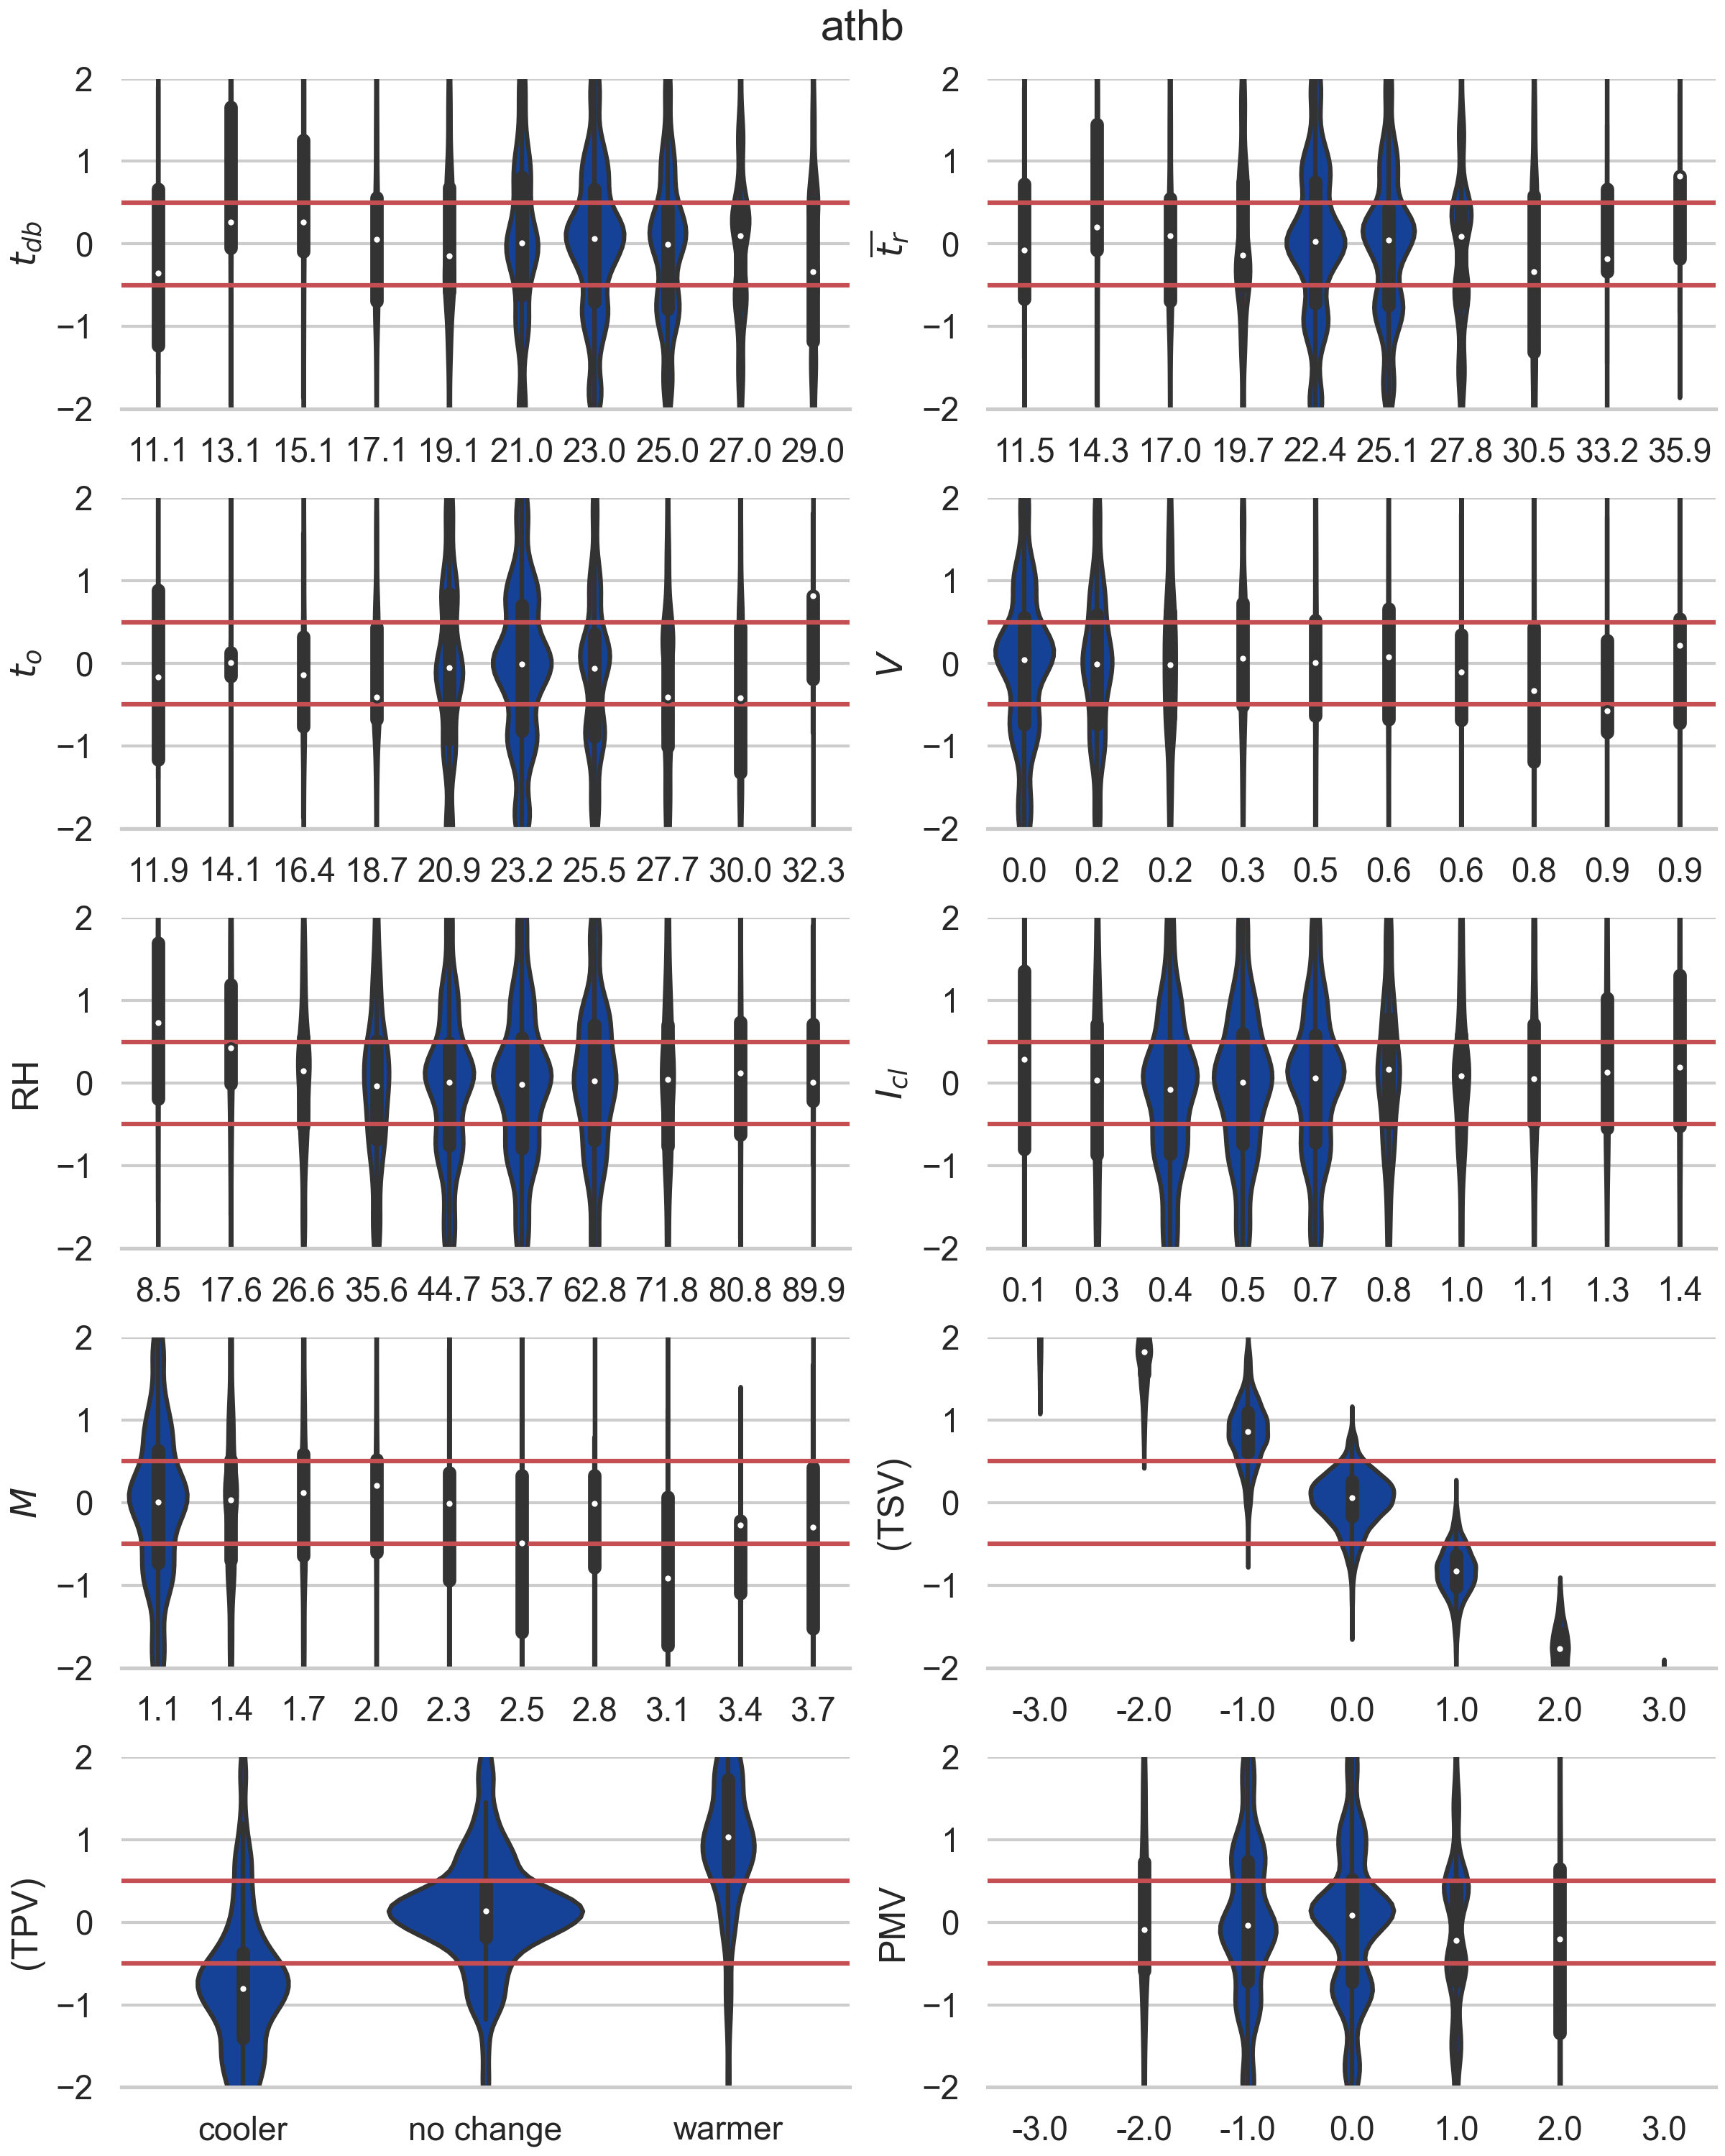
\includegraphics[width=\textwidth]{figures/bias_athb}
    \caption{}
    \label{fig:bias_athb}
\end{figure}